\documentclass[border=10pt]{standalone}

\usepackage{tikz}
\usepackage{tikzsymbols}
\usetikzlibrary{calc,patterns,shapes.geometric}

\def\centerarc[#1](#2)(#3:#4:#5){\draw[#1] ($(#2)+({#5*cos(#3)},{#5*sin(#3)})$) arc (#3:#4:#5);}

\begin{document}
	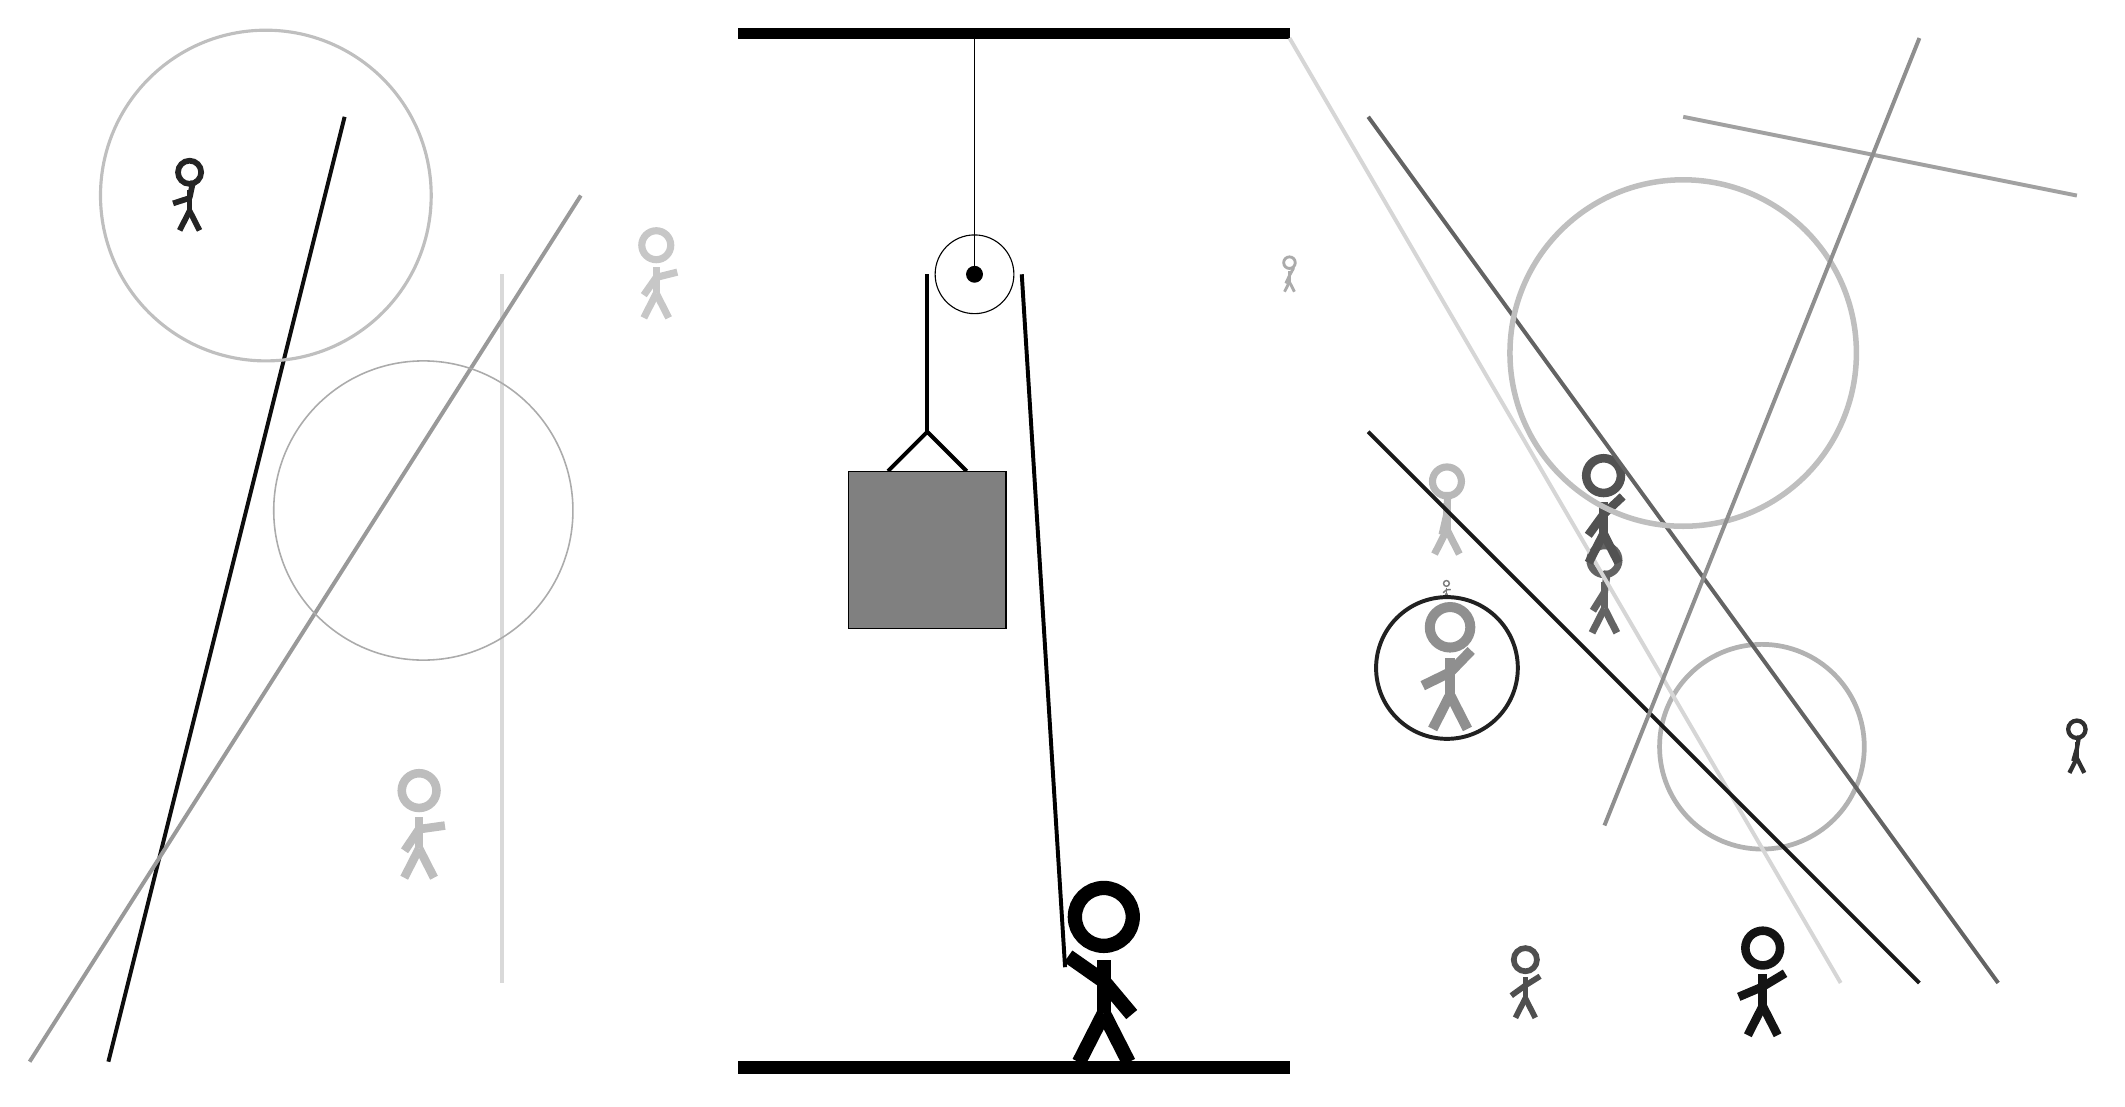
\begin{tikzpicture}
		%%%%% START %%%%%
		
		\draw[fill=black] (-2, 10) rectangle (5, 10.125);
		
		\draw (1, 7) circle (0.5);
		\draw[fill=black] (1, 7) circle (0.1);
		\draw (1, 10) -- (1, 7);
		
		\draw[line width=0.5mm] (-0.1, 4.5) -- (0.4, 5.0) -- (0.9, 4.5);
		\draw[fill=black!50] (-0.6, 4.5) rectangle (1.4, 2.5);
		
		\draw[line width=0.5mm] (0.4, 7) -- (0.4, 5.0);
		\centerarc[line width=0.5mm](1, 7)(0:180:0.6);
		\draw[line width=0.5mm](1.6, 7) -- (2.15, -1.8);
		
		\node at (2.6, -1.9) {\Strichmaxerl[10][-35][-50]};
		
		\node[line width=0.2mm, color=black!22] at (-3, 7) {\Strichmaxerl[5][55][14]};
		
		\node[line width=0.4mm, color=black!52] at (7, 3) {\Strichmaxerl[1][41][5]};
		\draw[line width=0.5mm, color=black!95](-7, 9) -- (-10, -3);
		\node[line width=0.7mm, color=black!61] at (9, 3) {\Strichmaxerl[5][58][82]};
		
		\draw [line width=0.6mm, color=black!30](11, 1) circle (1.3);
		\draw[line width=0.5mm, color=black!15](-5, 7) -- (-5, -2);
		\draw[line width=0.5mm, color=black!16](5, 10) -- (12, -2);
		\node[line width=0.4mm, color=black!28] at (7, 4) {\Strichmaxerl[5][77][88]};
		\draw[line width=0.5mm, color=black!37](10, 9) -- (15, 8);
		\draw [line width=0.5mm, color=black!87](7, 2) circle (0.9);
		\draw[line width=0.5mm, color=black!90](6, 5) -- (13, -2);
		\node[line width=0.2mm, color=black!69] at (8, -2) {\Strichmaxerl[4][36][32]};
		\node[line width=0.3mm, color=black!44] at (7, 2) {\Strichmaxerl[7][26][46]};
		\draw[line width=0.5mm, color=black!40](-4, 8) -- (-11, -3);
		\node[line width=0.7mm, color=black!26] at (-6, 0) {\Strichmaxerl[6][56][8]};
		\draw [line width=0.4mm, color=black!25](-8, 8) circle (2.1);
		\node[line width=0.3mm, color=black!68] at (9, 4) {\Strichmaxerl[6][54][43]};
		\node[line width=0.2mm, color=black!33] at (5, 7) {\Strichmaxerl[2][65][61]};
		\draw [line width=0.2mm, color=black!33](-6, 4) circle (1.9);
		\node[line width=0.6mm, color=black!86] at (-9, 8) {\Strichmaxerl[4][18][78]};
		\node[line width=0.2mm, color=black!92] at (11, -2) {\Strichmaxerl[6][23][31]};
		
		\node[line width=0.2mm, color=black!81] at (15, 1) {\Strichmaxerl[3][74][80]};
		\draw[line width=0.5mm, color=black!61](6, 9) -- (14, -2);
		\draw [line width=0.7mm, color=black!25](10, 6) circle (2.2);
		\draw[line width=0.5mm, color=black!44](9, 0) -- (13, 10);
		
		
		\draw[fill=black] (-2, -3) rectangle (5, -3.15);
		
		%%%%% END %%%%%
	\end{tikzpicture}
\end{document}